% ==============================================================================
% CAPITOLO 5: ANALISI DEI RISULTATI E DISCUSSIONE SPERIMENTALE
% ==============================================================================
\chapter{Analisi dei Risultati e Discussione Sperimentale}
\label{ch:risultati}

Il presente capitolo espone e analizza i risultati ottenuti mediante il protocollo
sperimentale implementato nel Capitolo~\ref{ch:implementazione}, ponendo particolare
attenzione alla capacità delle differenti configurazioni di classificazione di
mantenere un comportamento discriminativo stabile in presenza di variazioni del
dominio di traffico.

L'analisi viene condotta secondo una progressione coerente con il framework
metodologico definito nel Capitolo~\ref{ch:metodologia}. In primo luogo, viene
esaminata la struttura geometrica e distributiva dei benchmark mediante gli
strumenti diagnostici PCA e KDE, al fine di caratterizzare preliminarmente
l'entità dello scostamento tra il dominio sorgente e le configurazioni contenenti
traffico target. Successivamente, vengono valutate le prestazioni della baseline
\textit{INJECTION}, assunta come riferimento sperimentale, e confrontate
separatamente con quelle dei modelli addestrati esclusivamente sul dominio
sorgente e con quelle dei modelli ibridi.

La valutazione quantitativa viene sviluppata combinando i risultati puntuali
ottenuti per il seed rappresentativo $s=42$ con le statistiche aggregate sulle
$K=10$ repliche stocastiche definite nel protocollo \textit{multi-seed}. Tale
impostazione consente di distinguere la descrizione analitica delle singole
configurazioni dalla verifica della stabilità dei risultati rispetto
all'inizializzazione degli stimatori. Il confronto viene infine completato
mediante il test $t$ di Welch sull'\textit{F1-Score} e attraverso l'analisi
post-hoc SHAP delle caratteristiche maggiormente coinvolte nelle decisioni dei
classificatori.

La parte conclusiva del capitolo integra quindi le evidenze prestazionali,
distributive e di spiegabilità, con l'obiettivo di individuare associazioni
coerenti tra variazioni dello spazio delle caratteristiche e comportamento
predittivo. Le eventuali relazioni individuate vengono interpretate nei limiti
consentiti dagli artefatti sperimentali disponibili, distinguendo le evidenze
direttamente osservabili dalle possibili spiegazioni di carattere
trasmissivo e di rete.


% ==============================================================================
% SEZIONE 1: DIAGNOSTICA SPAZIALE E DISTRIBUTIVA
% ==============================================================================
\section{Diagnostica Spaziale e Distributiva}
\label{sec:diagnostica_spaziale_distributiva}

Prima di procedere alla valutazione quantitativa dei classificatori, risulta
necessario caratterizzare il modo in cui le differenti configurazioni di
benchmark occupano lo spazio condiviso delle caratteristiche $\mathcal{X}$.
A tale scopo vengono impiegati gli strumenti diagnostici implementati nella
Sezione~\ref{subsec:implementazione_pca_kde}, mantenuti rigorosamente separati
dal processo di addestramento e inferenza.

L'analisi considera tre configurazioni rappresentative dell'intero protocollo
sperimentale: il benchmark sorgente \texttt{NB15}, il benchmark di riferimento
\texttt{INJECTION} e il benchmark ibrido \texttt{NB15\_STIN}. Tale selezione
permette di osservare progressivamente il passaggio dalla distribuzione
puramente sorgente, alla condizione di adattamento sparso adottata dalla
baseline, fino alla configurazione nella quale la componente malevola è
interamente derivata dal dominio target.


% ------------------------------------------------------------------------------
% PCA
% ------------------------------------------------------------------------------
\subsection{Proiezioni PCA dello Spazio delle Feature}
\label{subsec:proiezioni_pca}

L'Analisi delle Componenti Principali viene utilizzata come strumento
diagnostico non supervisionato per osservare la disposizione dei campioni
all'interno di una rappresentazione bidimensionale dello spazio condiviso delle
$16$ \textit{feature}. Come definito nel Capitolo~\ref{ch:implementazione},
l'analisi viene condotta esclusivamente sulle partizioni di test e utilizza un
sistema di riferimento comune dipendente dal dominio sorgente.

In particolare, lo standardizzatore viene adattato sul benchmark sorgente
\texttt{NB15} e le statistiche $(\boldsymbol{\mu}_S,\boldsymbol{\sigma}_S)$
così ottenute vengono mantenute fisse durante la trasformazione delle
configurazioni successive. Analogamente, la matrice degli autovettori
$\mathbf{W}_S$ viene determinata una sola volta mediante il fitting della PCA
sul benchmark sorgente standardizzato. Ciascun generico benchmark $D$ viene
pertanto rappresentato secondo

\begin{equation}
    \mathbf{P}_D
    =
    \left(
    \frac{\mathbf{X}_D-\boldsymbol{\mu}_S}
    {\boldsymbol{\sigma}_S+\epsilon}
    \right)
    \mathbf{W}_S,
    \label{eq:cap5_pca_source_projection}
\end{equation}

senza alcun ricalcolo locale dello standardizzatore o degli assi principali.

Questa proprietà risulta essenziale per l'interpretazione dei grafici
successivi. La percentuale di varianza riportata sugli assi, pari al
$40{,}35\%$ per \texttt{PC1} e al $16{,}00\%$ per \texttt{PC2}, per una
varianza spiegata complessiva del $56{,}36\%$, si riferisce infatti alla PCA
adattata sul dominio sorgente. La medesima percentuale riportata nelle tre
figure non implica pertanto che \texttt{NB15}, \texttt{INJECTION} e
\texttt{NB15\_STIN} possiedano la stessa struttura di varianza; indica invece
che tutti i benchmark vengono osservati attraverso lo stesso sistema di
coordinate latenti definito da $\mathbf{W}_S$.

\begin{figure}[H]
    \centering
    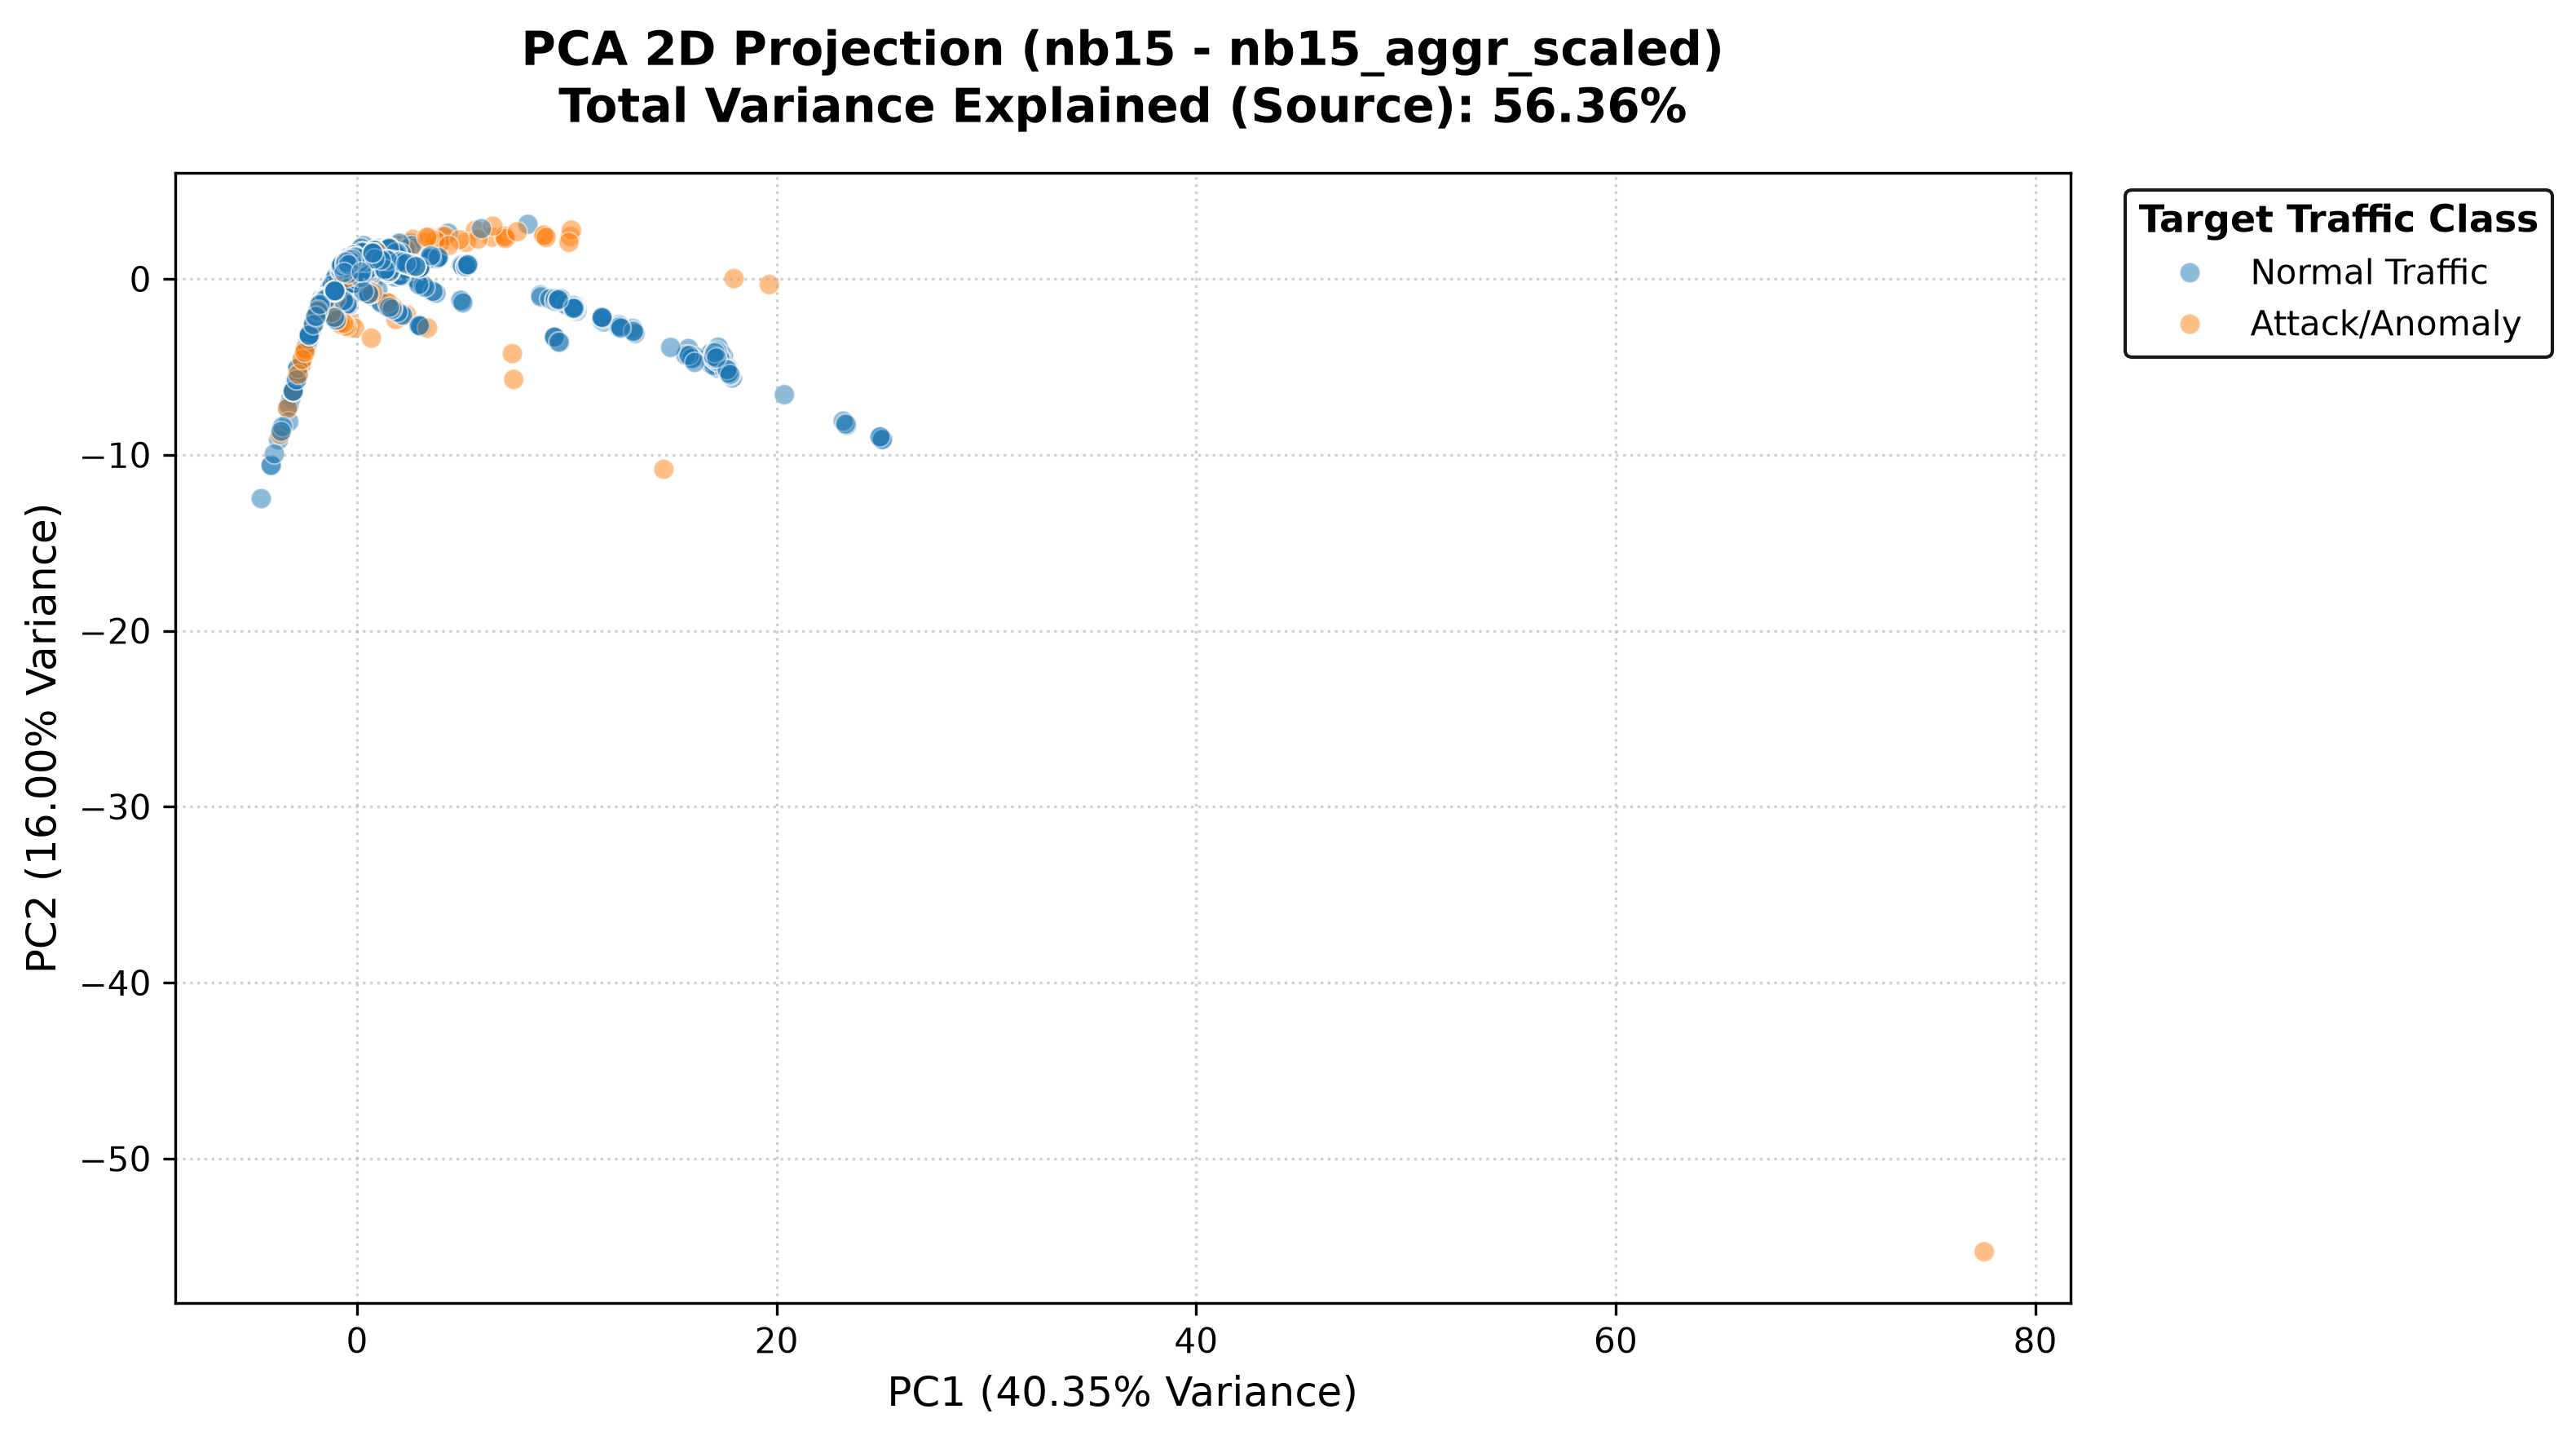
\includegraphics[width=0.95\textwidth]{images/chapter4/pca/pca_sorgente_nb15.png}
    \caption{Proiezione PCA bidimensionale del benchmark sorgente \texttt{NB15}
    nel sistema di riferimento ottenuto mediante standardizzazione e fitting
    sul dominio sorgente.}
    \label{fig:pca_sorgente_nb15}
\end{figure}

La Figura~\ref{fig:pca_sorgente_nb15} costituisce il riferimento geometrico
dell'analisi. La maggior parte delle osservazioni risulta concentrata in una
regione relativamente compatta del piano, caratterizzata da una struttura
curvilinea e da alcune estensioni periferiche lungo entrambe le componenti.
All'interno di tale regione è osservabile una consistente sovrapposizione tra
traffico nominale e traffico malevolo: i punti appartenenti alle due classi
occupano in larga misura le medesime porzioni dello spazio latente, mentre
alcune osservazioni anomale risultano collocate in regioni più periferiche.

La rappresentazione non evidenzia pertanto una separazione globale netta delle
due classi nelle sole prime due componenti principali. Tale risultato non
costituisce un'anomalia, poiché la PCA non utilizza l'etichetta $Y$ nella
costruzione degli assi e massimizza esclusivamente la varianza complessiva dei
dati. La sovrapposizione osservata indica quindi che una parte della struttura
discriminativa presente nello spazio originario non può essere ricondotta a
una semplice separazione lineare nel piano formato da \texttt{PC1} e
\texttt{PC2}.

\begin{figure}[H]
    \centering
    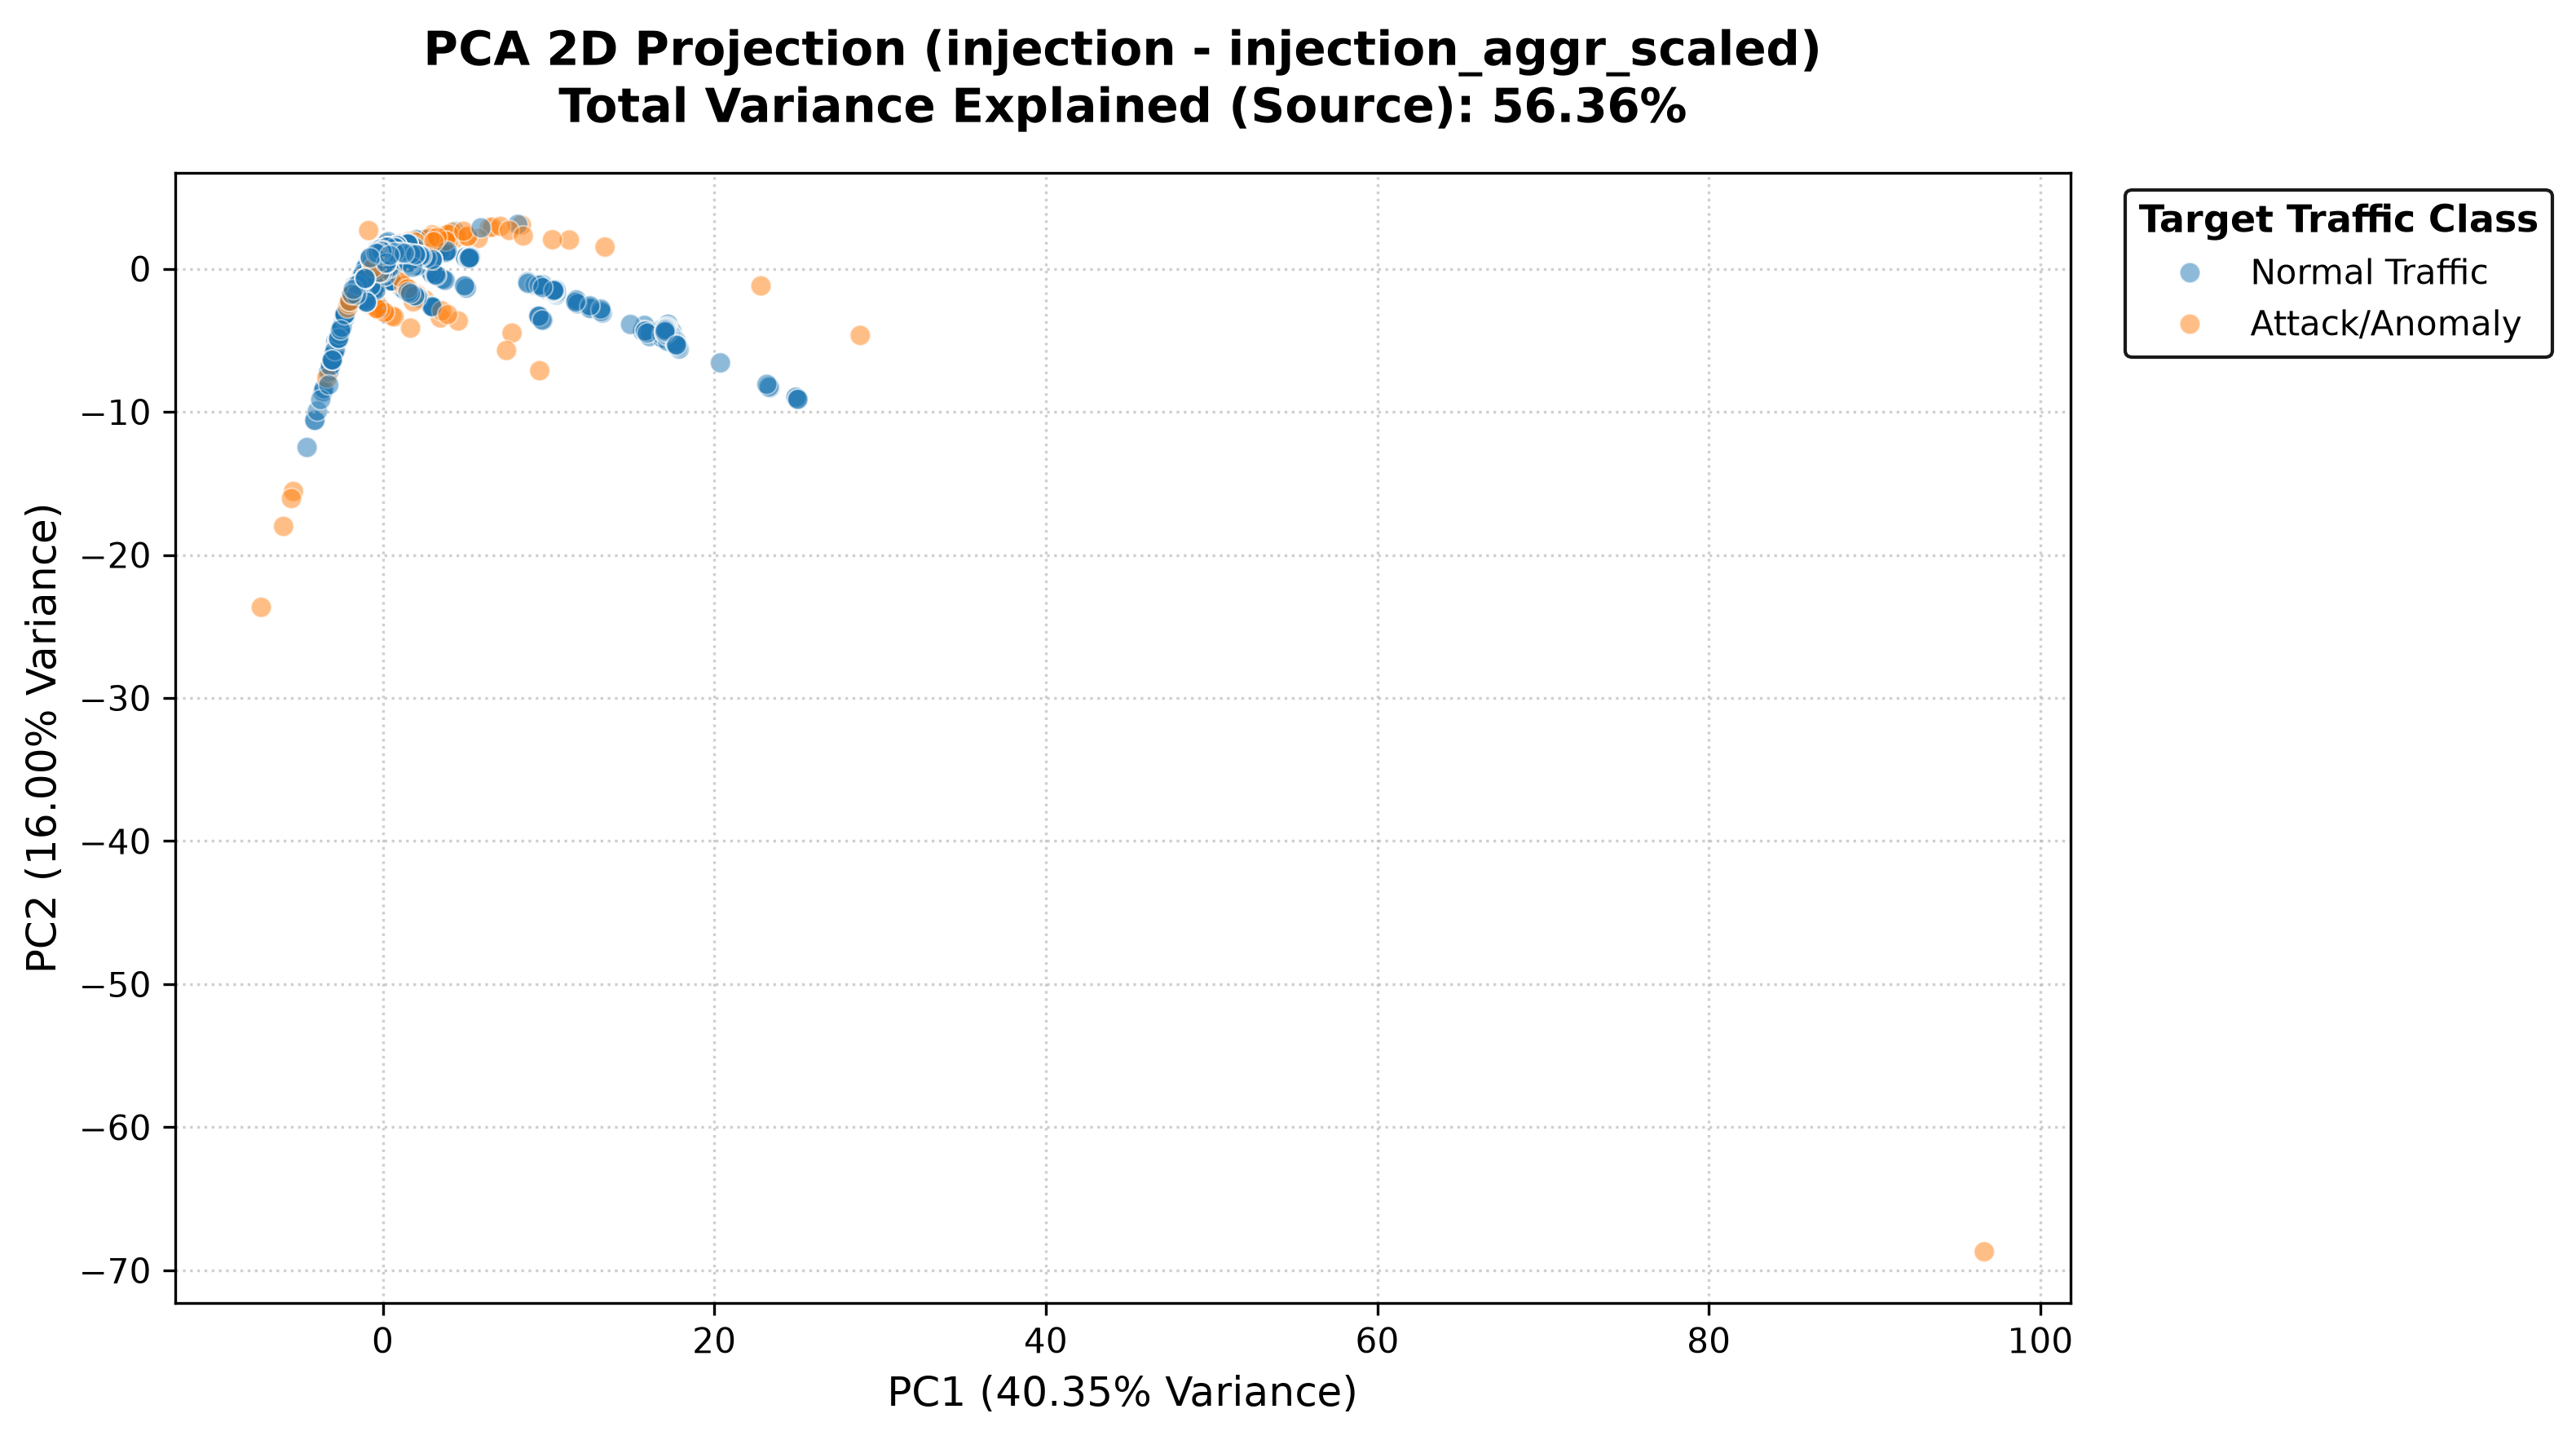
\includegraphics[width=0.95\textwidth]{images/chapter4/pca/pca_baseline_injection.png}
    \caption{Proiezione PCA bidimensionale del benchmark
    \texttt{INJECTION}, utilizzato per l'addestramento della baseline
    $\mathcal{M}_{\text{base}}$, nel sistema di riferimento PCA definito
    dal dominio sorgente.}
    \label{fig:pca_baseline_injection}
\end{figure}

La configurazione \texttt{INJECTION}, riportata nella
Figura~\ref{fig:pca_baseline_injection}, mantiene una struttura geometrica
complessivamente prossima a quella osservata per il benchmark sorgente.
Questo comportamento risulta coerente con la composizione del dataset:
la componente nominale deriva integralmente da \texttt{NB15}, mentre la
componente malevola è dominata dagli attacchi sorgente e incorpora soltanto
una quota target pari allo $0{,}3\%$ della popolazione malevola target
considerata nella procedura di iniezione.

Nel piano PCA permane infatti un'estesa sovrapposizione tra le due etichette
nella regione principale occupata dalla distribuzione sorgente. Contestualmente,
sono presenti osservazioni malevole collocate a distanza considerevole dal
nucleo principale e una maggiore estensione della regione periferica.
Il solo grafico non permette di associare individualmente tali osservazioni
alla componente \texttt{NB15} o alla quota \texttt{STIN} iniettata, poiché
la colorazione distingue esclusivamente la natura nominale o malevola del
campione e non il relativo dominio di provenienza. La presenza di tali
osservazioni periferiche deve pertanto essere considerata come evidenza
geometrica osservabile, senza attribuirne causalmente l'origine alla componente
target in assenza di un'etichettatura esplicita di dominio nel grafico.

\begin{figure}[H]
    \centering
    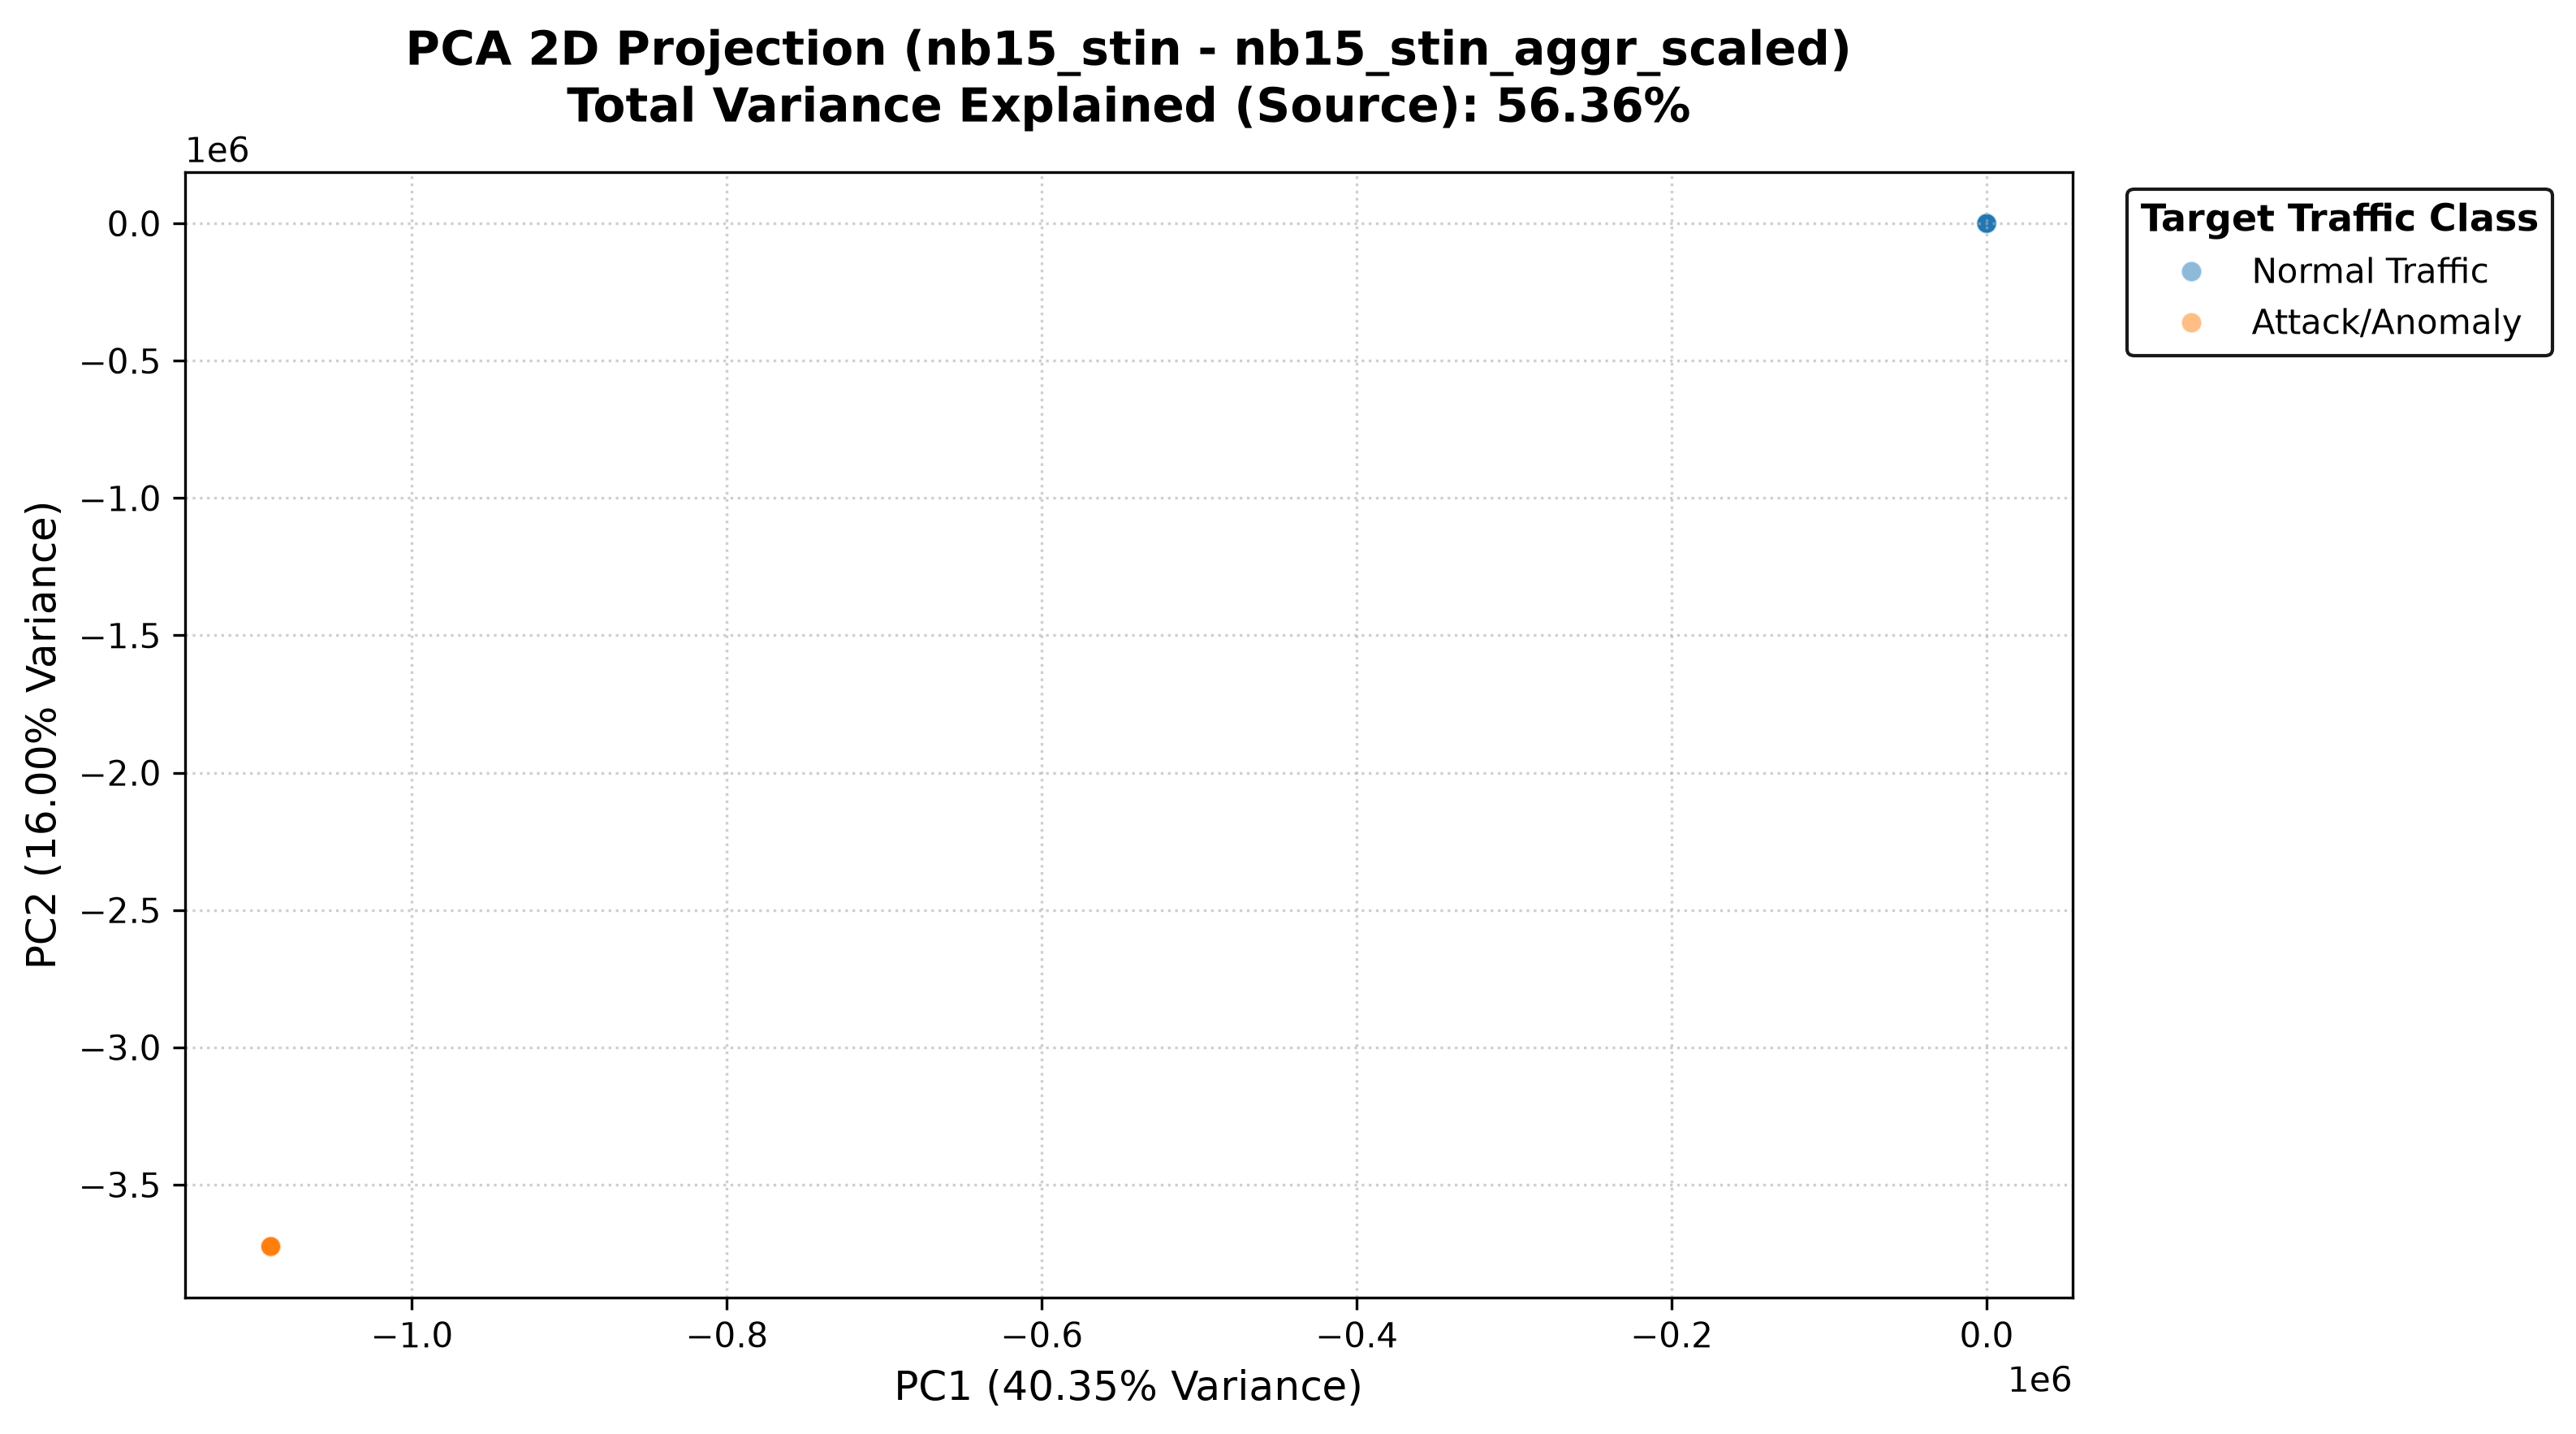
\includegraphics[width=0.95\textwidth]{images/chapter4/pca/pca_hybrid_nb15_stin.png}
    \caption{Proiezione PCA bidimensionale del benchmark ibrido
    \texttt{NB15\_STIN}, composto da traffico nominale sorgente
    \texttt{NB15} e traffico malevolo target \texttt{STIN}, nel sistema
    di riferimento PCA definito dal dominio sorgente.}
    \label{fig:pca_hybrid_nb15_stin}
\end{figure}

Una configurazione sostanzialmente differente emerge per il benchmark ibrido
\texttt{NB15\_STIN}, mostrato nella
Figura~\ref{fig:pca_hybrid_nb15_stin}. In questo caso, i vettori malevoli
\texttt{STIN} proiettati mediante lo standardizzatore e gli autovettori
ottenuti esclusivamente da \texttt{NB15} raggiungono coordinate di ordine
sensibilmente superiore rispetto a quelle occupate dal benchmark sorgente.
La scala del piano raggiunge infatti valori dell'ordine di $10^{6}$,
determinando una forte compressione visiva del traffico nominale sorgente
nell'intorno dell'origine.

Tale compressione non deve essere interpretata come una riduzione della
cardinalità dei campioni rappresentati. Essa costituisce un effetto della
scala grafica necessaria a rappresentare simultaneamente osservazioni che,
nel sistema di riferimento statistico del sorgente, occupano regioni
estremamente distanti. Il risultato rende quindi immediatamente visibile
l'elevata distanza geometrica tra la componente nominale \texttt{NB15} e la
componente malevola \texttt{STIN} all'interno delle direzioni di variabilità
apprese sul dominio sorgente.

L'interpretazione di tale separazione richiede tuttavia una distinzione
fondamentale. Nel benchmark \texttt{NB15\_STIN}, la variabile di classe e il
dominio di provenienza risultano strutturalmente associati: il traffico con
$Y=0$ deriva dal dominio sorgente \texttt{NB15}, mentre il traffico con $Y=1$
deriva dal dominio target \texttt{STIN}. Di conseguenza, la netta distanza
osservata nel piano PCA non può essere attribuita esclusivamente alla
separabilità tra traffico benigno e malevolo. Essa incorpora inevitabilmente
anche la variazione distributiva associata al passaggio dal dominio sorgente
al dominio target.

La Figura~\ref{fig:pca_hybrid_nb15_stin} fornisce pertanto una forte evidenza
diagnostica della presenza di uno scostamento rispetto al riferimento
sorgente, ma non consente, isolatamente, di separare la componente dovuta alla
natura malevola del traffico da quella associata alla diversa origine
distributiva dei campioni. Tale distinzione verrà approfondita mediante
l'analisi KDE delle singole caratteristiche e, successivamente, attraverso
l'analisi SHAP del comportamento dei classificatori.

Nel complesso, il confronto tra le tre proiezioni delinea una progressione
geometrica coerente con le differenti modalità di composizione dei benchmark.
Il dominio \texttt{NB15} definisce il manifold di riferimento; la
configurazione \texttt{INJECTION} ne preserva sostanzialmente la struttura
dominante introducendo una perturbazione target estremamente sparsa; il
benchmark \texttt{NB15\_STIN}, al contrario, espone direttamente il modello
diagnostico alla componente malevola target, determinando uno scostamento
di diversi ordini di grandezza nello spazio PCA ancorato al sorgente.
Questa evidenza costituisce il primo indicatore sperimentale della rilevanza
del \textit{domain shift} che verrà successivamente messo in relazione con
le distribuzioni marginali delle feature e con le prestazioni dei
classificatori.

% ------------------------------------------------------------------------------
% KDE E DOMAIN SHIFT
% ------------------------------------------------------------------------------
\subsection{Stime di Densità di Kernel (KDE) e Domain Shift}
\label{subsec:stime_kde}

L'analisi geometrica condotta mediante PCA viene affiancata da un'ispezione
distributiva a livello delle singole caratteristiche tramite
\textit{Kernel Density Estimation} (KDE). Mentre la proiezione PCA fornisce una
rappresentazione sintetica dell'intero spazio delle feature, la KDE consente di
osservare direttamente come specifiche variabili discriminanti modifichino la
propria distribuzione al passaggio dal dominio sorgente alle configurazioni
contenenti traffico target.

Coerentemente con il protocollo definito nei
Capitoli~\ref{ch:metodologia} e~\ref{ch:implementazione}, l'analisi viene
ristretta alle tre caratteristiche selezionate mediante il procedimento di
aggregazione delle evidenze SHAP:
\texttt{pkts\_per\_sec}, \texttt{total\_bytes} e
\texttt{dst\_win\_byt}. Per ciascuna variabile, i valori vengono espressi nel
sistema standardizzato dipendente dal sorgente definito
nell'Equazione~\eqref{eq:z_score_source}. Una coordinata $z=0$ corrisponde
pertanto alla media della relativa feature nel benchmark sorgente, mentre uno
scostamento positivo o negativo esprime la distanza rispetto a tale riferimento
in unità della deviazione standard sorgente.

A differenza della procedura PCA, la routine KDE implementata nel
Capitolo~\ref{ch:implementazione} non applica un filtraggio esplicito sulla
colonna \texttt{split\_type}. Le distribuzioni rappresentate nelle figure
seguenti descrivono quindi il benchmark complessivamente considerato e non la
sola partizione di test. Tale distinzione non modifica la finalità diagnostica
dell'analisi, ma deve essere mantenuta esplicita nell'interpretazione dei
risultati.

Le densità relative al traffico nominale e malevolo sono inoltre normalizzate
indipendentemente mediante l'impostazione \texttt{common\_norm=False}.
Di conseguenza, l'altezza relativa delle due curve non deve essere interpretata
come indicatore della diversa numerosità delle classi. L'interesse analitico
risiede invece nella posizione, nell'estensione, nella forma e nel grado di
sovrapposizione dei rispettivi supporti. Analogamente, l'asse verticale in
scala \texttt{symlog} consente di rendere osservabili anche regioni a densità
molto ridotta senza modificarne l'ordinamento distributivo.


\begin{figure}[H]
    \centering
    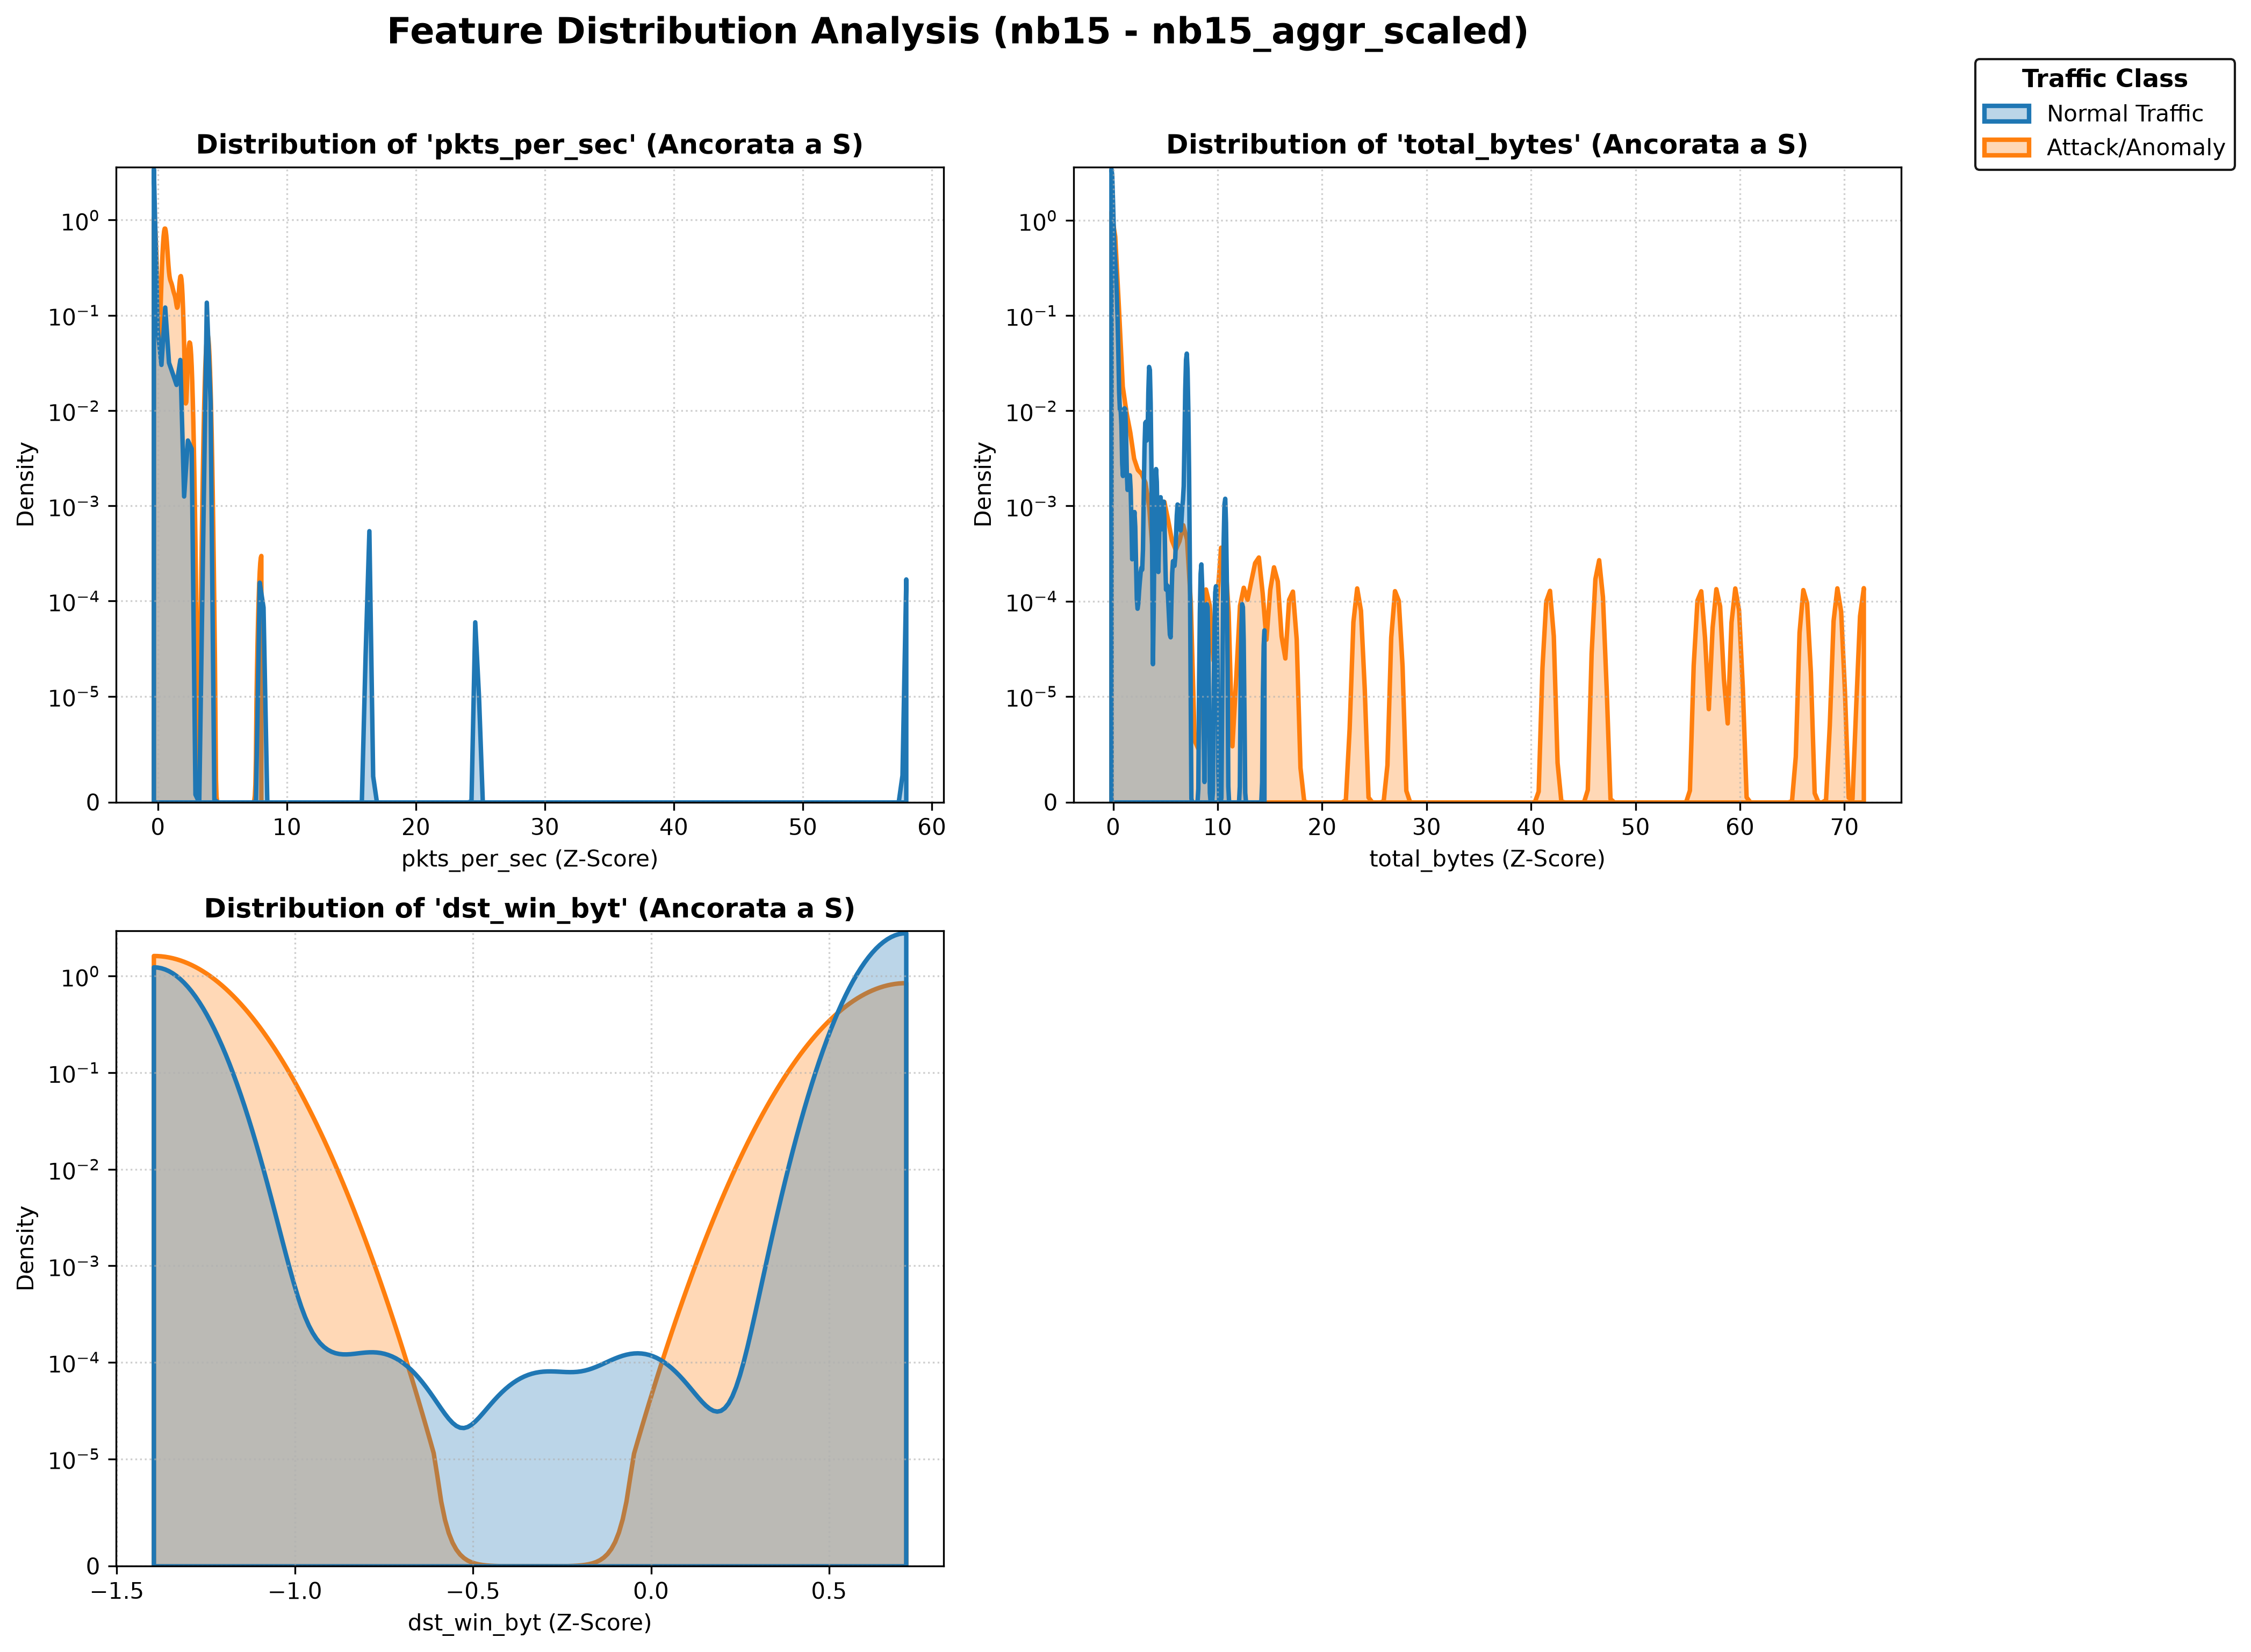
\includegraphics[width=\textwidth]{images/chapter4/kde/kde_sorgente_nb15.png}
    \caption{Stime KDE delle feature \texttt{pkts\_per\_sec},
    \texttt{total\_bytes} e \texttt{dst\_win\_byt} per il benchmark
    sorgente \texttt{NB15}, espresse mediante standardizzazione ancorata
    al dominio sorgente.}
    \label{fig:kde_sorgente_nb15}
\end{figure}

La Figura~\ref{fig:kde_sorgente_nb15} costituisce il riferimento distributivo
iniziale. Per la feature \texttt{pkts\_per\_sec}, entrambe le classi presentano
la maggiore concentrazione in prossimità dell'origine dello spazio
standardizzato. La regione principale mostra una sovrapposizione consistente
tra traffico nominale e malevolo, accompagnata dalla presenza di componenti a
densità inferiore distribuite verso valori positivi di Z-score. La classe
nominale presenta, in particolare, alcune estensioni periferiche anche a
distanze elevate rispetto alla media sorgente. La sola
\texttt{pkts\_per\_sec} non determina quindi, nel dominio \texttt{NB15}, una
separazione distributiva completa tra le due etichette.

Un comportamento differente emerge per \texttt{total\_bytes}. Sebbene entrambe
le distribuzioni mantengano una regione ad elevata concentrazione in
prossimità dell'origine, la componente malevola presenta numerose estensioni
verso valori positivi dello spazio standardizzato, raggiungendo regioni non
occupate con analoga continuità dalla distribuzione nominale. Questa
asimmetria indica che, all'interno del dominio sorgente, una parte del traffico
malevolo è associata a configurazioni di volume complessivo sensibilmente
differenti rispetto al nucleo principale del traffico nominale.

Per \texttt{dst\_win\_byt} viene invece osservata una struttura marcatamente
bimodale. Le distribuzioni delle due classi mostrano concentrazioni in
prossimità degli estremi dell'intervallo standardizzato e un'ampia regione
intermedia caratterizzata da densità ridotte. La sovrapposizione tra traffico
nominale e malevolo rimane significativa in entrambe le regioni principali,
sebbene la forma delle curve non risulti perfettamente coincidente. Nel
benchmark sorgente tale feature descrive pertanto una struttura distributiva
complessa, ma non una separazione univoca delle classi.


\begin{figure}[H]
    \centering
    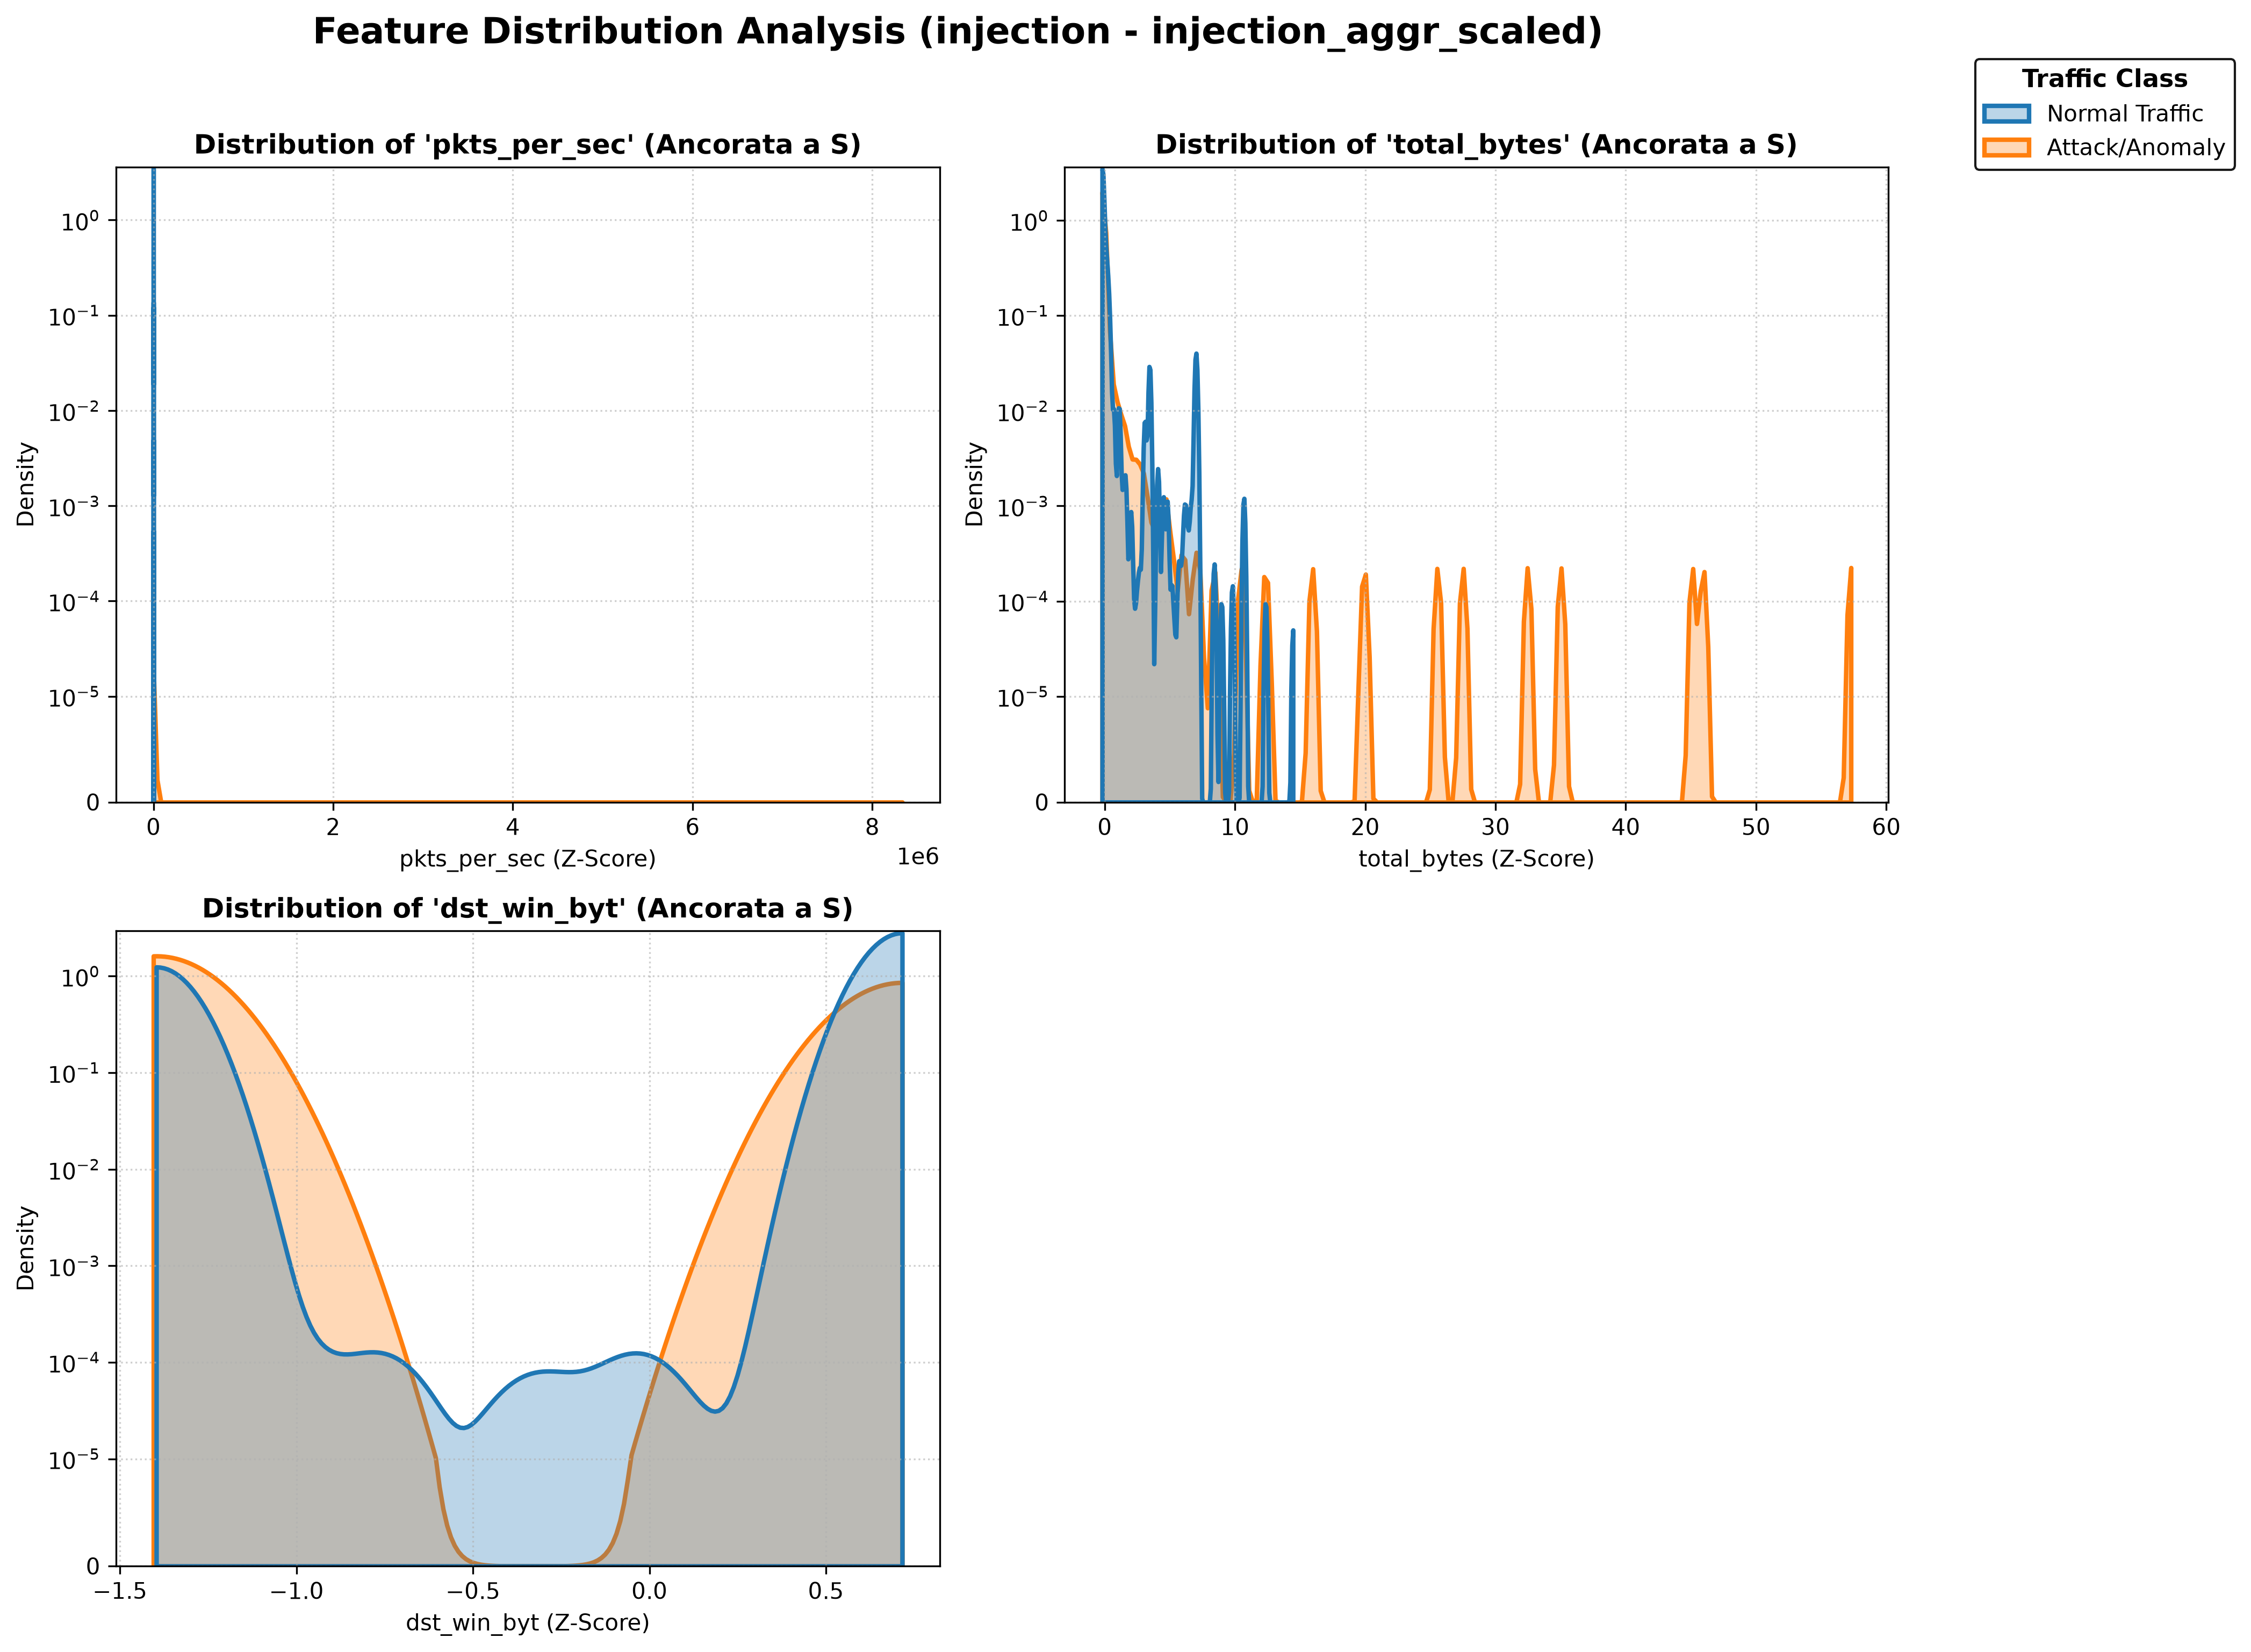
\includegraphics[width=\textwidth]{images/chapter4/kde/kde_baseline_injection.png}
    \caption{Stime KDE delle feature \texttt{pkts\_per\_sec},
    \texttt{total\_bytes} e \texttt{dst\_win\_byt} per il benchmark
    \texttt{INJECTION}, utilizzato per l'addestramento della baseline
    $\mathcal{M}_{\text{base}}$.}
    \label{fig:kde_baseline_injection}
\end{figure}

La configurazione \texttt{INJECTION}, mostrata nella
Figura~\ref{fig:kde_baseline_injection}, preserva per
\texttt{total\_bytes} e \newline \texttt{dst\_win\_byt} una morfologia
distributiva complessivamente prossima a quella del dominio sorgente. Tale
risultato è coerente con la composizione del benchmark di riferimento, nel
quale la componente nominale è interamente derivata da \texttt{NB15} e la
componente malevola rimane prevalentemente sorgente, con una contaminazione
target limitata allo $0{,}3\%$ della popolazione malevola target prevista dal
protocollo di iniezione.

La differenza più evidente rispetto alla
Figura~\ref{fig:kde_sorgente_nb15} interessa
\texttt{pkts\_per\_sec}. La distribuzione malevola conserva una regione
principale prossima all'origine, ma introduce contestualmente una coda
estremamente estesa verso valori positivi, che raggiunge Z-score dell'ordine
di $10^{6}$. Una simile coordinata non deve essere interpretata come valore
grezzo della variabile, bensì come distanza rispetto alla media e alla
deviazione standard definite esclusivamente sul sorgente. La sua ampiezza
indica quindi che alcune osservazioni contenute in \texttt{INJECTION} risultano
fortemente esterne al supporto caratteristico di \texttt{NB15} per questa
specifica feature.

Il confronto diretto con il benchmark sorgente rende tale evidenza
particolarmente significativa. La coda di questa ampiezza non è osservabile
nella distribuzione \texttt{NB15}, mentre compare nel benchmark ottenuto
mediante l'inserimento controllato dei campioni target. Considerata la
composizione nota dei due dataset, tale variazione risulta coerente con
l'introduzione della componente \texttt{STIN}. Tuttavia, la ridotta densità
associata alla regione periferica conferma contestualmente il carattere sparso
dell'iniezione: la struttura dominante del benchmark continua infatti a
rimanere prossima a quella sorgente.

Per \texttt{total\_bytes}, la baseline conserva il comportamento caratterizzato
da una regione comune in prossimità dell'origine e da estensioni positive
prevalentemente associate alla classe malevola. Analogamente,
\texttt{dst\_win\_byt} mantiene la struttura bimodale osservata in
\texttt{NB15}, con un'elevata sovrapposizione tra le due classi. Nel complesso,
la configurazione \texttt{INJECTION} appare quindi prevalentemente ancorata
alla struttura distributiva sorgente, pur introducendo segnali localizzati
compatibili con la conoscenza target sparsa incorporata nel benchmark.


\begin{figure}[H]
    \centering
    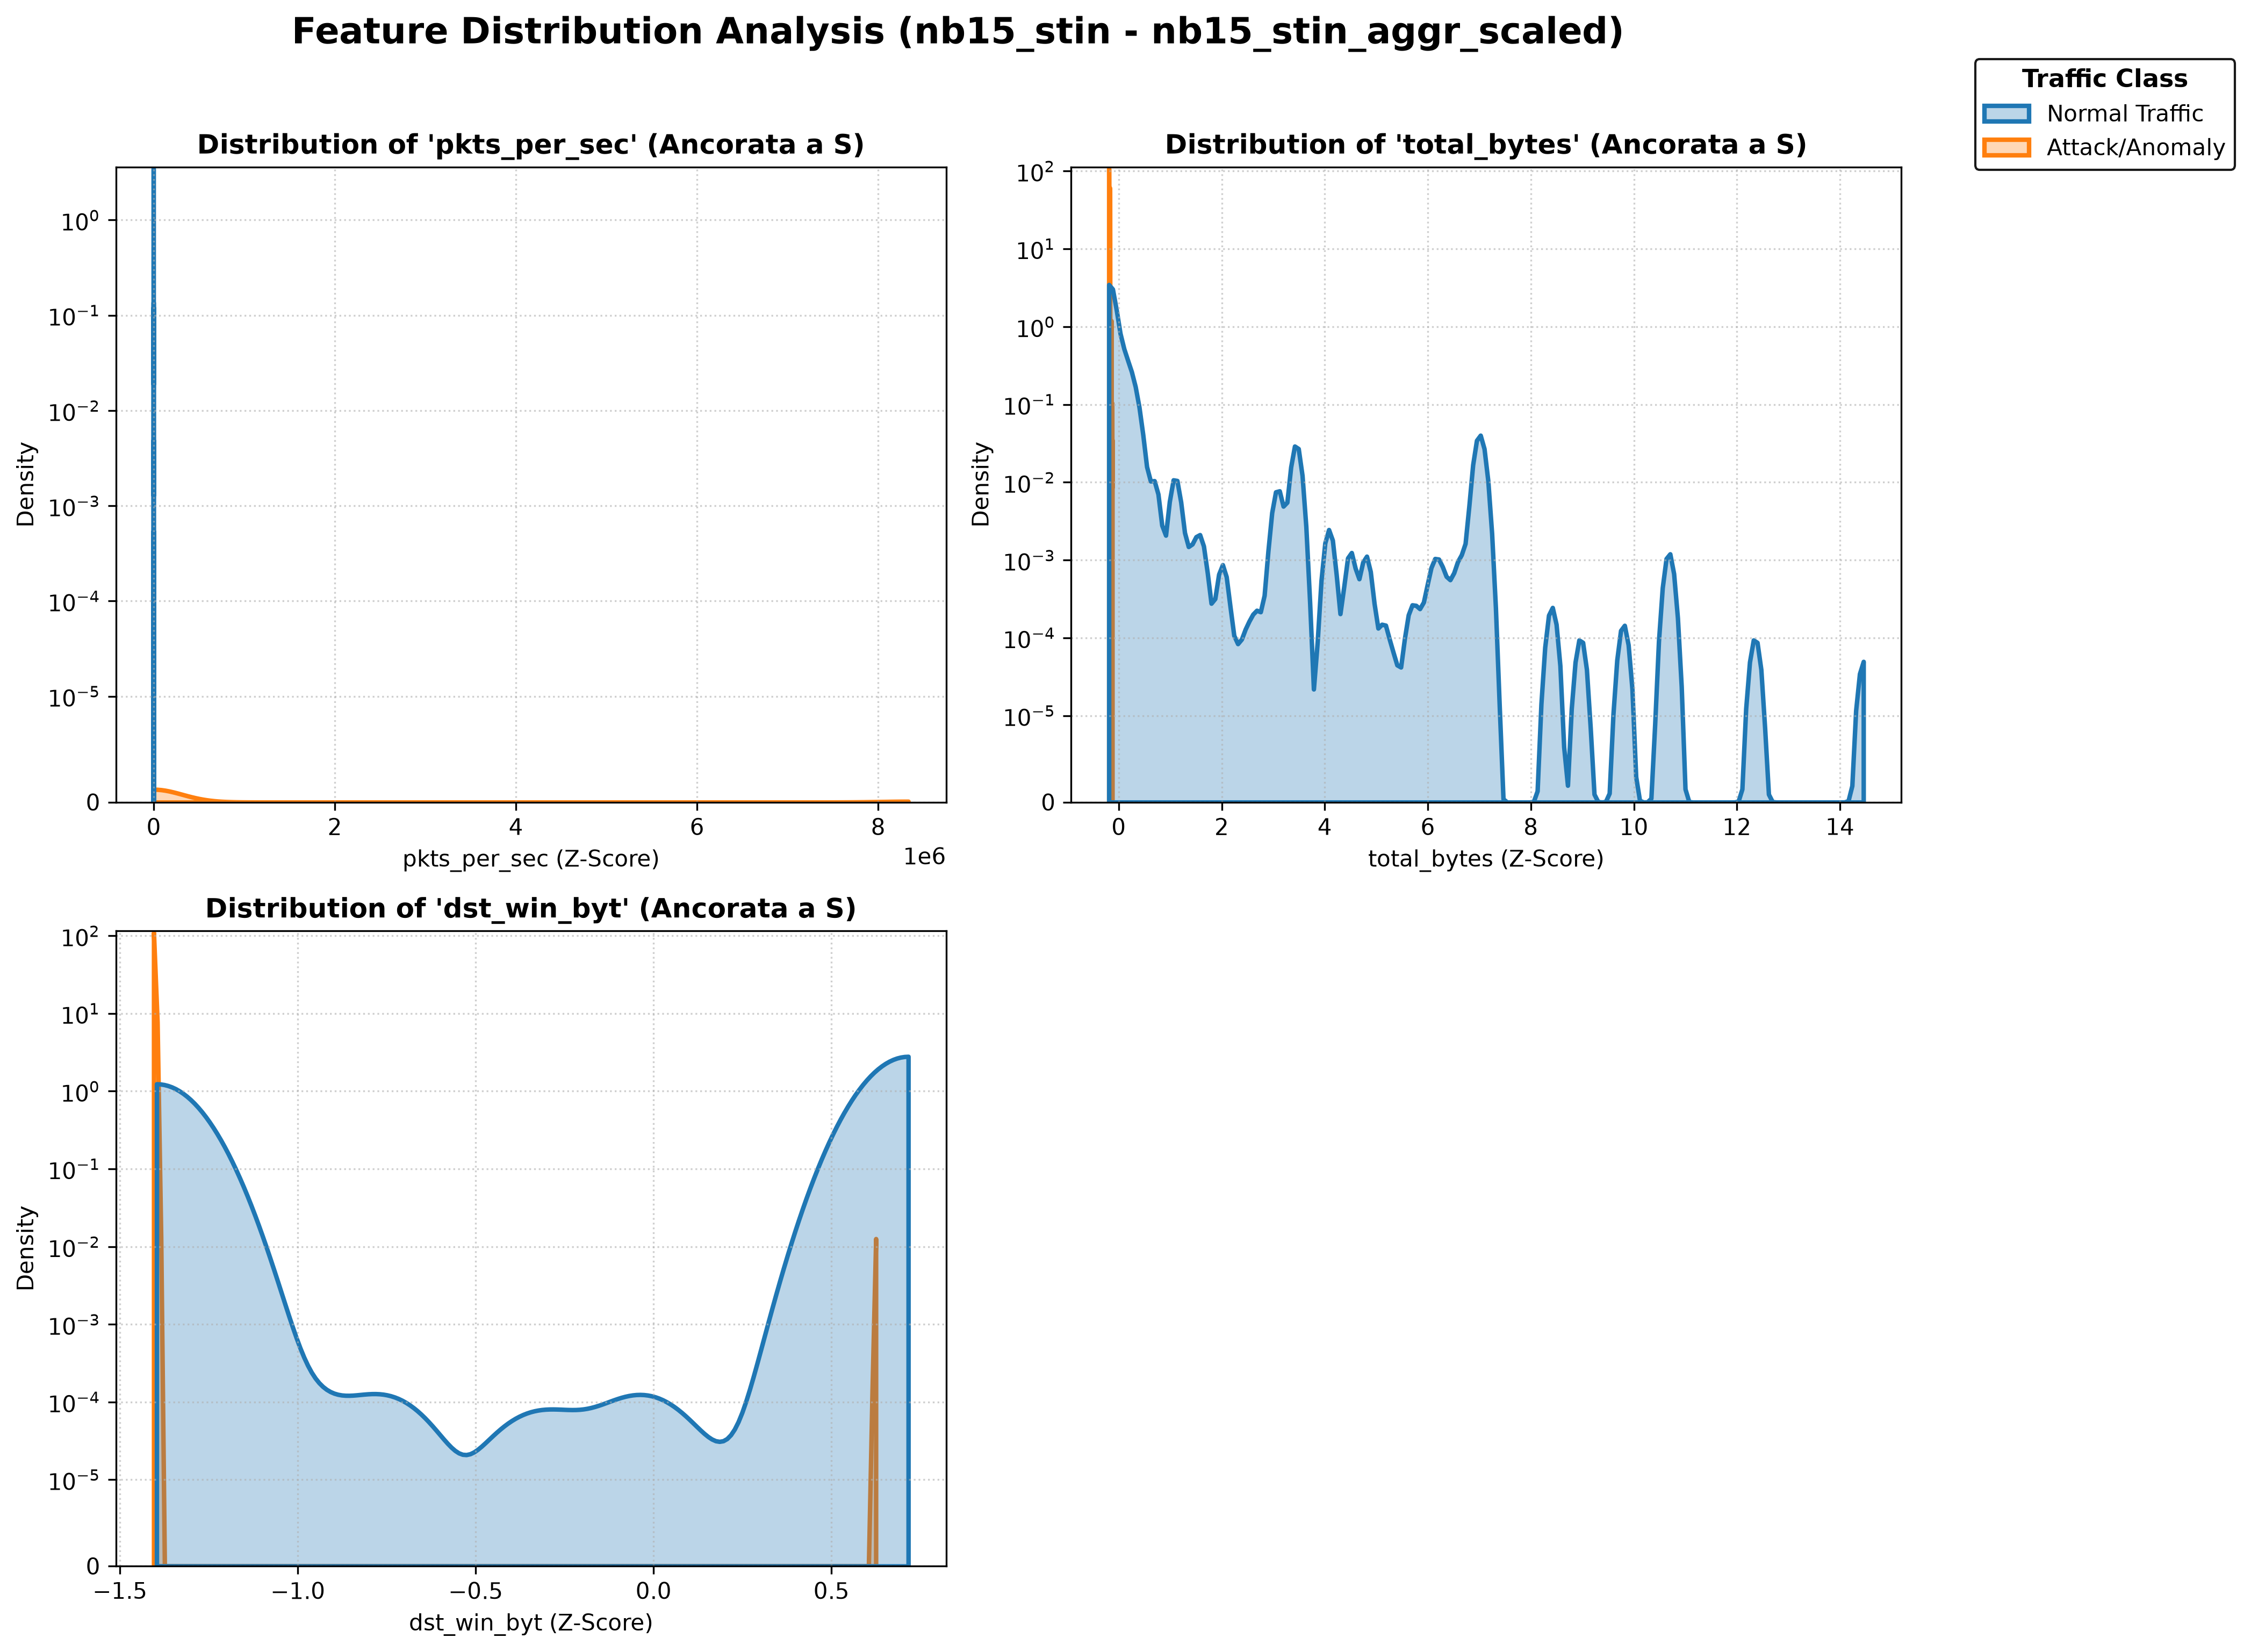
\includegraphics[width=\textwidth]{images/chapter4/kde/kde_hybrid_nb15_stin.png}
    \caption{Stime KDE delle feature \texttt{pkts\_per\_sec},
    \texttt{total\_bytes} e \texttt{dst\_win\_byt} per il benchmark
    ibrido \texttt{NB15\_STIN}, costituito da traffico nominale sorgente
    \texttt{NB15} e traffico malevolo target \texttt{STIN}.}
    \label{fig:kde_hybrid_nb15_stin}
\end{figure}

Il passaggio al benchmark ibrido \texttt{NB15\_STIN}, riportato nella
Figura~\ref{fig:kde_hybrid_nb15_stin}, determina una modificazione
distributiva sensibilmente più pronunciata. In questa configurazione la
componente nominale continua a provenire dal dominio sorgente, mentre l'intera
componente malevola è sostituita dal traffico target \texttt{STIN}. Il
confronto con le due figure precedenti consente pertanto di osservare come le
tre feature selezionate reagiscano alla sostituzione completa della
distribuzione anomala sorgente con quella target.

La caratteristica \texttt{pkts\_per\_sec} rappresenta l'evidenza più marcata.
La distribuzione nominale rimane concentrata in prossimità del riferimento
sorgente, mentre quella associata agli attacchi \texttt{STIN} si estende su
un intervallo positivo dell'ordine di milioni di deviazioni standard sorgente.
La scala orizzontale necessaria a contenere questi valori comprime
visivamente la distribuzione nominale nell'intorno dell'origine, in modo
analogo a quanto osservato nella proiezione PCA del benchmark ibrido.

Questa evidenza è compatibile con un severo \textit{covariate shift} nella
feature \texttt{pkts\_per\_sec}: i campioni target assumono valori che, dopo
l'applicazione dello stesso operatore di armonizzazione
$\boldsymbol{\psi}_T$ e dello stesso riferimento statistico sorgente,
risultano collocati molto al di fuori della regione caratteristica di
\texttt{NB15}. L'elevata magnitudine degli Z-score non rappresenta quindi,
isolatamente, un'anomalia della procedura di standardizzazione. Al contrario,
l'assenza di un ricentramento locale preserva deliberatamente lo scostamento
rispetto a $(\mu_S,\sigma_S)$ che una standardizzazione indipendente del
benchmark target avrebbe occultato.

Una dinamica differente viene osservata per \texttt{total\_bytes}. Nel
benchmark sorgente e nella baseline la classe malevola mostrava diverse
estensioni verso valori positivi elevati. Nel benchmark
\texttt{NB15\_STIN}, al contrario, la densità degli attacchi target risulta
fortemente concentrata in una regione ristretta prossima al riferimento
sorgente, mentre la distribuzione nominale \texttt{NB15} mantiene un supporto
positivo decisamente più esteso. La sostituzione della componente malevola
modifica pertanto non soltanto l'ampiezza della distribuzione, ma anche la
relazione relativa tra le due classi lungo questa dimensione.

Il risultato risulta rilevante perché mostra come il \textit{domain shift} non
si manifesti necessariamente attraverso una traslazione concorde di tutte le
feature verso valori estremi. Nel caso di \texttt{pkts\_per\_sec}, la
differenza tra sorgente e target assume la forma di una forte espansione del
supporto; per \texttt{total\_bytes}, essa emerge invece dalla differente
concentrazione e disposizione relativa delle densità. La variazione di dominio
deve pertanto essere interpretata come trasformazione multidimensionale della
distribuzione $P(\mathbf{x})$, e non come un semplice spostamento uniforme
delle caratteristiche.

Anche \texttt{dst\_win\_byt} evidenzia una modifica strutturale. La componente
nominale conserva la distribuzione ampia e bimodale già osservata nel
benchmark sorgente, mentre i campioni malevoli \texttt{STIN} risultano
concentrati in regioni molto più ristrette, prossime agli estremi dello
spazio occupato dalla feature. Le elevate densità locali mostrate dalla curva
malevola non corrispondono a una maggiore numerosità degli attacchi, poiché le
KDE delle due classi sono normalizzate indipendentemente; esse indicano invece
una maggiore concentrazione della probabilità stimata in intervalli ridotti
della caratteristica.

Considerando congiuntamente le tre feature, il confronto tra
\texttt{NB15}, \texttt{INJECTION} e \texttt{NB15\_STIN} evidenzia quindi tre
condizioni distributive distinte. Il benchmark sorgente definisce il
riferimento statistico e presenta differenti livelli di sovrapposizione tra
traffico nominale e malevolo. La baseline \texttt{INJECTION} conserva in larga
parte tale struttura, ma introduce una componente periferica particolarmente
evidente in \texttt{pkts\_per\_sec}. Il benchmark ibrido, infine, manifesta
una trasformazione molto più pronunciata delle distribuzioni associate alla
classe malevola, coerentemente con la sostituzione completa degli attacchi
sorgente mediante attacchi \texttt{STIN}.

Le evidenze KDE risultano inoltre coerenti, sul piano diagnostico, con quanto
osservato mediante PCA. L'estrema separazione del benchmark
\texttt{NB15\_STIN} nel piano delle prime due componenti principali trova
infatti un riscontro diretto nell'ampiezza dello scostamento osservato almeno
su \texttt{pkts\_per\_sec}, mentre le distribuzioni di
\texttt{total\_bytes} e \texttt{dst\_win\_byt} mostrano che il cambiamento
di dominio coinvolge anche la forma e la concentrazione delle distribuzioni,
non esclusivamente la loro posizione.

Tale corrispondenza non implica tuttavia che le tre feature KDE siano, da sole,
responsabili della geometria osservata mediante PCA, poiché quest'ultima è
calcolata sull'intero spazio condiviso delle $16$ caratteristiche. Le due
analisi devono essere considerate complementari: la PCA evidenzia
globalmente la presenza di una differente collocazione geometrica del traffico,
mentre la KDE permette di identificare specifiche dimensioni lungo le quali lo
scostamento distributivo risulta direttamente osservabile.

La diagnostica ottenuta in questa sezione stabilisce pertanto il contesto
distributivo necessario per l'analisi prestazionale successiva. In
particolare, la presenza di differenze rilevanti tra le distribuzioni sorgente
e target rende necessario verificare se la conoscenza target estremamente
sparsa incorporata nella baseline \texttt{INJECTION} sia sufficiente a
mantenere adeguati livelli di rilevamento sui differenti benchmark. Tale
aspetto viene esaminato nella sezione seguente mediante la valutazione
quantitativa di $\mathcal{M}_{\text{base}}$ per le tre architetture di
classificazione considerate.

% ==============================================================================
% SEZIONE 2: VALUTAZIONE DELLA BASELINE INJECTION
% ==============================================================================
\section{Valutazione della Baseline INJECTION}
\label{sec:baseline_prestazioni}

% ------------------------------------------------------------------------------
% SPECIFICHE:
% Analisi del modello aggregato injection (M_base).
% Invece di dividere per algoritmo, presentare tabelle sinottiche comparative che 
% pongono a confronto diretto Decision Tree (DT), Histogram-based Gradient 
% Boosting (HGB) e Random Forest (RF) per ciascuna metrica sui 16 test set:
%   - nb15 (aggregato e biclasse: DoS, Exploits, Fuzzers, Generic, Reconnaissance)
%   - injection (aggregato)
%   - nb15_stin (aggregato)
%   - nb15_sat20 (aggregato e biclasse Syn_DDoS, UDP_DDoS)
%   - nb15_ter20 (aggregato e biclasse Botnet, DDoS, Syn_DDoS, UDP_DDoS)
% Metriche da mostrare: TP, TN, FP, FN, Precision, TPR, TNR, F1-Score, PR-AUC.
% ------------------------------------------------------------------------------

\subsection{Prestazioni Quantitative del Modello di Baseline}
\label{subsec:baseline_prestazioni_comparative}
% Tabelle comparative per DT, HGB e RF testati sui 16 test set descritti in precedenza.

\subsection{Analisi di Spiegabilità SHAP della Baseline INJECTION}
\label{subsec:baseline_shap}


% ==============================================================================
% SEZIONE 3: VALUTAZIONE DEI MODELLI SORGENTE ED IMPATTO DEL DOMAIN SHIFT
% ==============================================================================
\section{Valutazione dei Modelli Sorgente rispetto alla Baseline}
\label{sec:risultati_modelli_sorgente}

% ------------------------------------------------------------------------------
% SPECIFICHE:
% Analisi dell'impatto diretto del domain shift sui modelli addestrati 
% esclusivamente sul dominio sorgente M_S (UNSW-NB15).
% ------------------------------------------------------------------------------

\subsection{Prestazioni dei Modelli Biclasse e Aggregato Sorgente}
\label{subsec:sorgente_prestazioni_biclasse_aggregati}
% Tabelle comparative per DT, HGB e RF testati sui 16 test set descritti in precedenza.

\subsection{Analisi Comparativa Incrociata: Modelli Sorgente vs Baseline}
\label{subsec:analisi_incrociata_sorgente_baseline}

\subsection{Analisi SHAP del Modello Aggregato Sorgente NB15}
\label{subsec:sorgente_shap}

\subsection{Analisi della Significatività Statistica (Test t di Welch) dei Modelli Sorgente vs Baseline}
\label{subsec:sorgente_welch_ttest}
% Analisi delle medie dell'F1-Score (F1-Score_means) calcolate sui diversi seed 
% e presentazione dei p-value ottenuti dal test t di Welch per DT, HGB e RF.


% ==============================================================================
% SEZIONE 4: VALUTAZIONE DEI MODELLI IBRIDI
% ==============================================================================
\section{Valutazione dei Modelli Ibridi rispetto alla Baseline}
\label{sec:risultati_modelli_ibridi}

% ------------------------------------------------------------------------------
% SPECIFICHE:
% Analisi dei modelli addestrati combinando i dati del dominio sorgente e target 
% per superare i limiti del domain shift.
% ------------------------------------------------------------------------------

\subsection{Prestazioni dei Modelli Biclasse e Aggregati Ibridi}
\label{subsec:ibridi_prestazioni}
% Tabelle comparative DT, HGB e RF testati sui 16 test set descritti in precedenza.

\subsection{Analisi Comparativa Incrociata: Modelli Ibridi vs Baseline}
\label{subsec:analisi_incrociata_ibridi_baseline}

\subsection{Analisi SHAP del Modello Aggregato Ibrido NB15\_STIN}
\label{subsec:ibridi_shap}

\subsection{Analisi della Significatività Statistica (Test t di Welch) dei Modelli Ibridi vs Baseline}
\label{subsec:ibridi_welch_ttest}
% Analisi delle medie dell'F1-Score (F1-Score_means) calcolate sui diversi seed 
% e presentazione dei p-value ottenuti dal test t di Welch per DT, HGB e RF.


% ==============================================================================
% SEZIONE 5: DISCUSSIONE GENERALE E CONFRONTO SINOTTICO
% ==============================================================================
\section{Discussione Generale e Quadro Comparativo Globale}
\label{sec:discussione_generale}

% ------------------------------------------------------------------------------
% SPECIFICHE:
% Sintesi finale che mette in relazione M_S, M_base e M_H.
% ------------------------------------------------------------------------------

\subsection{Quadro Comparativo Globale}
\label{subsec:quadro_comparativo_globale}
% Tabella riassuntiva finale con i risultati chiave dei tre paradigmi a confronto.

\subsection{Mappatura Causa-Effetto tra Proprietà della Rete e Comportamento del Modello}
\label{subsec:sintesi_causa_effetto}

\subsection{Compromesso tra Complessità Computazionale e Prestazioni}
\label{subsec:tradeoff_complessita_prestazioni}

\subsection{Considerazioni Operative per l'Applicabilità in Ambito NIDS Satellitare}
\label{subsec:implicazioni_operative_nids}


% ==============================================================================
% SEZIONE 6: CONCLUSIONI DEL CAPITOLO
% ==============================================================================
\section{Sintesi e Conclusioni del Capitolo}
\label{sec:cap5_conclusioni}
% Sintesi dei messaggi chiave emersi dagli esperimenti e ponte verso il capitolo 
% conclusivo della tesi.

